\chapter{UML}\label{chap:uml}
\section{Modélisation}
\begin{definition}[Modèle]
    Un modèle est une représentation simplifiée d’une partie de la réalité dans un but spécifique.
\end{definition}
Un modèle est toujours une abstraction: pour réduire la complexité, on ne tient pas compte de certaines caractéristiques ou propriétés de l’objet complexe qu’on modélise, afin de se concentrer sur d’autres.

\begin{itemize}
    \item Exactitude: dévelopez des modèles syntaxiquement corrects
    \item Précision: évitez l’ambiguité dans les modèles 
    \item Concision: évitez les détails inutiles
    \item Complétude: modélisez tous les aspects essentiels 
    \item Cohérence: évitez les incohérences dans les modèles
    \item Compréhensibilité: créez des modèles lisibles et compréhensibles
    \item Uniformité: utilisez un style uniforme partout
\end{itemize}


\begin{definition}[UML — Unified Modeling Language]
    UML (Unified Modeling Language) est un ensemble de notations pour décrire un système logiciel de manière visuelle en termes de modèles (Langage de modélisation).
\end{definition}


\begin{table}[H]
	\centering
		\caption{Langage UML}
		\label{tbl:modélisation}
		\begin{adjustbox}{max width=\textwidth}
		\begin{tabular}{l|l|l}
			\toprule
			\multirow{6}{*}{Points Forts}&\multirow{3}{*}{Langage \og semi-formel\fg et standardisé}		&  Gain de précision\\
			\cmidrule(lr){3-3}
            & & Gage de stabilité\\
            \cmidrule(lr){3-3}
            & & Encourage l’automatisation via l’utilisation d’outils dédiés\\
            \cmidrule(lr){2-2}\cmidrule(lr){3-3}
            &\multirow{3}{*}{Support de communication efficace}
			&  Cadre l'analyse des besoins\\
			\cmidrule(lr){3-3}
            & & Facilite la compréhension de systèmes abstrait et complexes\\
            \cmidrule(lr){3-3}
            & & Langage universel car polyvalent et souple\\
			%\midrule
            \cmidrule{1-2} \cmidrule(lr){3-3}
			\multirow{4}{*}{Points Faibles}& \multirow{2}{*}{Nécessité d'apprentissage et de période d’adaptation} 
			& UML contient beaucoup (trop?) de diagrammes ...  \\
			\cmidrule(lr){3-3}
			&& On peut commencer avec un sous-ensemble \\
			\cmidrule(lr){2-2}\cmidrule(lr){3-3}
			&\multirow{2}{*}{Absence du processus, clé de la réussite d’un projet}
			& Intégration d'UML dans un processus $\implies Difficile$\\
			\cmidrule(lr){3-3}
			&& Améliorer un processus est une tâche longue et complexe\\
			\bottomrule
		\end{tabular}
		\end{adjustbox}
\end{table}

\begin{table}[H]
\centering
%\begin{center}
\caption{Catégories et sous-catégories de diagrammes UML}
\label{tbl:uml}
\begin{adjustbox}{max width=\textwidth}
\begin{tabular}{p{7em}|p{6em}|p{14em}|p{35em}}
\toprule

\multicolumn{2}{}{Modélisation} & Type de diagramme & Description \\
\midrule

\multirow{6}{}{Structure Statique} & \multirow{4}{}{Objet}& \nameref{sec:diagrammeclasse} & Décrit les classes, leurs interrelations, et leurs instances. \\
\cmidrule(lr){3-4}
&& Diagramme d'objets & Décrit les objets et leurs relations avec les classes. \\
\cmidrule(lr){3-4}
&& Diagramme de paquetages & Montre la répartition des éléments dans des groupes logiques. \\
\cmidrule(lr){3-4}
&& Composite structure diagram & Représente la structure interne de composants de logiciel. \\
\cmidrule(lr){2-4}
&\multirow{2}{}{Architecture} & Diagramme de composants (logiciel) & Montre comment les différents composants du logiciel sont organisés logiquement. \\
\cmidrule(lr){3-4}
&& Diagramme de déploiement (matériel) & Montre comment les différents composants du matériel (hardware) sont organisés physiquement. \\
\cmidrule(lr){1-4}


\multirow{7}{}{Comportement Dynamique} & \multirow{1}{}{Utilisation} & \nameref{sec:diagrammecasutilisation} & Montre les utilisations possibles d'un logiciel.\\
\cmidrule(lr){2-4}
&\multirow{2}{}{Activités et États} & \nameref{sec:diagrammeetatscomportementaux} & Montre comment le système se comporte de façon interne, modélise le comportement discret piloté par les évènements.\\
\cmidrule(lr){3-4}
&& \nameref{sec:diagrammeactivite} & Modélise le comportement d’un système ou processus basé sur les flux de contrôle.\\
\cmidrule(lr){2-4}
&\multirow{4}{}{Interaction} & \nameref{sec:diagrammesequence} & Montre le comportement du système par l’interaction des objets qui le compose.\\
\cmidrule(lr){3-4}
&& Diagramme de communication & Montre comment les objets communiquent entre eux.\\
\cmidrule(lr){3-4}
&& \nameref{sec:diagrammeinteraction} & Montre comment les processus et interactions sont organisés dans le système.\\
\cmidrule(lr){3-4}
&& Timing diagram & Montre comment les interactions et les changements d'états sont liés dans le temps.\\
\bottomrule
\end{tabular}
\end{adjustbox}
%\end{center}
\end{table}





\newpage
\section{Diagramme de Cas d'Utilisation (Use Case Diagram)}\label{sec:diagrammecasutilisation}
\begin{definition}[Diagramme de Cas d'Utilisation]
Un diagramme de cas d'utilisation est un type de diagramme UML qui représente les interactions entre un système et ses utilisateurs dans le but de réaliser une fonctionnalité spécifique.

Un diagramme de cas d’utilisation:
\begin{itemize}
\item partitionne les besoins du système en différent cas d’utilisation
\item permet d’identifier des besoins contradictoires et des
imprécisions
\item permet d’identifier les rôles joués par les utilisateurs du
système; des utilisateurs différents ont des besoins différents
\end{itemize}

Un cas d'utilisation est une description des interactions entre un système et ses utilisateurs dans le but de réaliser une tâche spécifique. Il permet de décrire les besoins du système de manière structurée, de déterminer les rôles des utilisateurs et de comprendre les différents cas d'utilisation du système.



Un diagramme de cas d'utilisation est un outil de modélisation qui représente les interactions entre un système et ses utilisateurs pour atteindre un objectif spécifique. Il est utilisé pour identifier et spécifier les besoins du système en les partitionnant en différents cas d'utilisation, en identifiant les rôles joués par les utilisateurs et en repérant les besoins contradictoires et les imprécisions.

Un diagramme de cas d'utilisation est un type de diagramme UML qui représente les interactions entre les utilisateurs (acteurs) et un système. Ces diagrammes permettent de décrire les scénarios d'utilisation d'un système, c'est-à-dire les actions et les réactions du système face aux demandes des utilisateurs. Ils permettent également de définir les limites du système et de comprendre les interactions entre les différents acteurs et le système. Les diagrammes de cas d'utilisation sont souvent utilisés pour la modélisation de l'utilisation d'un système et peuvent être utilisés pour développer des spécifications fonctionnelles.
\end{definition}
\begin{definition}[Cas d'utilisation]
Un cas d'utilisation est une description des interactions entre un système et ses utilisateurs dans le but de réaliser une tâche spécifique. Il permet de décrire les besoins du système de manière structurée, de déterminer les rôles des utilisateurs et de comprendre les différents cas d'utilisation du système.
\end{definition}
\begin{definition}[Cas d'utilisation d'extension]
Un cas d'utilisation d'extension est une spécification qui décrit un cas d'utilisation qui peut étendre ou modifier le comportement d'un cas d'utilisation principal en cas de conditions exceptionnelles ou conditionnelles. Ces cas d'utilisation d'extension permettent de maintenir la simplicité de la description du cas d'utilisation principal en séparant les exceptions spécifiques.
\end{definition}

Un diagramme de cas d'utilisation est un type de diagramme UML qui représente les interactions entre les acteurs et le système en vue de réaliser une tâche spécifique. Il est composé de symboles tels que :
\begin{itemize}
\item Les acteurs : représentés par des personnes ou des entités extérieures au système
\item Les cas d'utilisation : représentés par des ellipses et décrivant une fonctionnalité du système
\item Les liens : représentés par des flèches reliant les acteurs aux cas d'utilisation et indiquant la relation de déclenchement ou d'interaction
\item Les conditions d'extension : représentées par des traits en pointillé reliant un cas d'utilisation principal à un cas d'utilisation d'extension et indiquant une fonctionnalité supplémentaire qui peut être réalisée dans certains cas spéciaux.
\end{itemize}

\newpage
\section{Diagramme d'Activités}\label{sec:diagrammeactivite}
\begin{definition}[Diagramme d'Activit\'es]
Un diagramme d'activité est un type de diagramme UML qui représente le flux de contrôle d'un processus ou d'un système en utilisant des symboles tels que des activités, des décisions et des transitions. Il permet de visualiser et de modéliser les différentes étapes d'un processus, les rôles des différents acteurs et les interactions entre ces différents éléments.

Un diagramme d'activité est un type de diagramme UML qui représente le comportement dynamique d'un système en décrivant la succession des activités nécessaires pour réaliser une certaine tâche, en mettant l'accent sur le flux de contrôle. Les diagrammes d'activités sont particulièrement utiles pour modéliser la fonctionnalité d'un système et pour présenter une vue dynamique de celui-ci.

Un diagramme d'activité est un type de diagramme UML qui représente le comportement d'un système ou processus en mettant en évidence les flux de contrôle et les actions qui sont réalisées. Il utilise des symboles tels que des boîtes pour représenter les actions et des flèches pour représenter le flux de contrôle entre ces actions. Les diagrammes d'activité sont utilisés pour modéliser les processus métier et les algorithmes, ainsi que pour analyser et optimiser les performances des systèmes. Ils peuvent également être utilisés pour décrire les interactions entre les différents éléments d'un système et pour déterminer comment ces éléments coopèrent pour atteindre un objectif commun. Enfin, les diagrammes d'activité sont souvent utilisés pour documenter les processus et les protocoles de travail, afin de faciliter la communication et la collaboration au sein d'une équipe.
\end{definition}
Voici la syntaxe générale d'un diagramme d'activités :
\begin{itemize}
\item L'acteur est représenté par un personnage avec une tête en forme de boîte.
\item Les activités sont représentées par des rectangles avec des bords arrondis. Elles peuvent être numérotées pour indiquer leur ordre d'exécution.
\item Les transitions entre les activités sont représentées par des flèches. Elles peuvent être annotées avec des conditions ou des événements qui déclenchent la transition.
\item Les décisions sont représentées par des losanges. Elles sont annotées avec une condition qui détermine la branche à suivre.
\item Les jonctions sont représentées par des cercles. Elles permettent de regrouper plusieurs transitions en une seule.
\item Les objets du système sont représentés par des boîtes avec un titre. Ils peuvent être utilisés pour indiquer les données manipulées par les activités.
\end{itemize}
Il existe également d'autres éléments qui peuvent être utilisés dans un diagramme d'activités, tels que les sous-activités, les points de synchronisation, les parallélismes, etc.



\newpage
\section{Diagramme d'Interaction (Interaction Overview Diagram)}\label{sec:diagrammeinteraction}

\begin{definition}[Diagramme d'interaction]
Un diagramme d'interaction est un type de diagramme UML qui représente les interactions entre les objets d'un système, en mettant en évidence leur comportement et les messages échangés.

Un diagramme d'interaction est un type de diagramme UML utilisé pour représenter et modéliser les interactions et les échanges de messages entre les différents éléments d'un système. Ces éléments peuvent être des objets, des classes, des composants, etc. Le diagramme d'interaction permet de visualiser la séquence des évènements qui se déroulent au cours d'une interaction entre ces éléments, ainsi que les conditions qui déclenchent ces évènements. Il permet également de décrire les rôles joués par chaque élément dans l'interaction et les obligations qu'il doit remplir. Le diagramme d'interaction est particulièrement utile pour comprendre et documenter le comportement dynamique d'un système.
\end{definition}

La syntaxe générale d'un diagramme d'interaction comprend les éléments suivants:
\begin{itemize}
\item Acteurs: représentés par des boîtes avec des têtes en forme de personnages, ils représentent les différents rôles joués par les utilisateurs du système.
\item Objets: représentés par des boîtes avec des titres, ils représentent les différents objets du système qui interagissent entre eux.
\item Messages: représentés par des flèches, ils indiquent l'envoi et la réception de messages entre les objets et les acteurs.
\item Répliques: représentées par des flèches en pointillés, elles indiquent les réponses des objets aux messages reçus.
\end{itemize}


\newpage
\section{Diagramme de Classe}\label{sec:diagrammeclasse}

\begin{definition}[Diagramme de Classe]
Un diagramme de classe est un type de diagramme UML qui représente les classes d'un système, leurs attributs et leurs méthodes, ainsi que leurs relations avec d'autres classes.

Un diagramme de classe est un type de diagramme UML qui représente les classes d'un système ainsi que leurs relations et leurs attributs. Il permet de visualiser la structure statique d'un système en modélisant ses différents objets et leurs interactions.

Un diagramme de classe est un type de diagramme UML qui représente les classes d'un système et leurs relations. Il permet de modéliser la structure statique du système en décrivant les classes, leurs attributs et leurs méthodes. Un diagramme de classe peut également illustrer les relations entre les classes, comme l'héritage, l'association ou l'agrégation. Un diagramme de classe est utile pour comprendre comment le système est organisé et comment les différentes parties interagissent entre elles. Il peut également être utilisé pour développer et maintenir le code source d'un projet logiciel.
\end{definition}

La syntaxe générale d'un diagramme de classes comprend les éléments suivants :
\begin{itemize}
\item Classe: représentée par une boîte avec un titre, elle décrit les propriétés et les comportements d'un type d'objet.
\item Attribut: représenté par un rectangle à l'intérieur de la classe, il décrit une propriété de l'objet.
\item Méthode: représentée par un rectangle avec un triangle à l'intérieur, elle décrit un comportement de l'objet.
\item Association: représentée par une flèche entre deux classes, elle indique que les objets de ces classes peuvent interagir entre eux.
\item Aggrégation: représentée par une flèche avec un diamant à la pointe, elle indique que l'objet d'une classe contient des objets d'une autre classe.
\item Composition: représentée par une flèche avec un cercle à la pointe, elle indique que l'objet d'une classe est dépendant des objets d'une autre classe.
\item Héritage: représenté par une flèche avec une croix à la pointe, il indique que la classe enfant hérite des propriétés et comportements de la classe parente.
\item Interfaces: représentées par des boîtes avec un titre souligné, elles décrivent les comportements attendus des objets qui implémentent cette interface.
\end{itemize}




\subsection{Composants}

\begin{table}[h]
\caption{Composants d'une classe en UML 2.5}
\label{tbl:class_components}
\begin{adjustbox}{max width=\textwidth}
\begin{tabular}{l|l}
\toprule
\textbf{Composant} & \textbf{Description} \\
\midrule
Nom de la classe & Le nom de la classe, qui doit être unique et décrire de manière concise la fonction de la classe. \\
%\cmidrule{1-2}
Visibilité & La visibilité de la classe, qui peut être publique, protégée ou privée. \\
%\cmidrule{1-2}
Modificateurs & Les modificateurs de la classe, tels que « abstract » ou « final ». \\
%\cmidrule{1-2}
Attributs & Les attributs de la classe, qui sont des variables membres qui décrivent les caractéristiques de la classe. \\
%\cmidrule{1-2}
Opérations & Les opérations de la classe, qui sont des méthodes membres qui décrivent les actions que la classe peut effectuer. \\
%\cmidrule{1-2}
Associations & Les associations de la classe, qui décrivent les relations entre la classe et d'autres classes ou objets. \\
%\cmidrule{1-2}
Dépendances & Les dépendances de la classe, qui décrivent les relations de dépendance entre la classe et d'autres classes ou objets. \\
%\cmidrule{1-2}
Notes & Les notes de la classe, qui sont des informations supplémentaires sur la classe. \\
\bottomrule
\end{tabular}
\end{adjustbox}
\end{table}
\subsubsection{Attributs}

\begin{table}[H]
\caption{Types d'attributs et de leur syntaxe en UML 2.5 :}
\label{tbl:class_attributs}
\begin{adjustbox}{max width=\textwidth}
\begin{tabular}{p{3cm}|p{2cm}|p{2cm}|l}
\toprule
\textbf{Type d'attribut} & \textbf{Symbole} & \textbf{Syntaxe} & \textbf{Description} \\
\midrule
Attribut public & $+$ & $+nom: type$ & L'attribut est accessible à l'extérieur de la classe. \\
%\cmidrule(lr){1-4}
Attribut protégé & $\#$ & $\#nom: type$ & L'attribut est accessible seulement par les classes héritant de la classe contenant l'attribut. \\
%\cmidrule(lr){1-4}
Attribut privé & $-$ & $-nom: type$ & L'attribut est accessible seulement à l'intérieur de la classe. \\
%\cmidrule(lr){1-4}
Attribut de package & $\textasciitilde$ & $\textasciitilde nom: type$ & L'attribut est accessible par toutes les classes dans le même package. \\
\bottomrule
\end{tabular}
\end{adjustbox}
\end{table}

\subsubsection{Opérations}

\begin{tabular}{p{3cm}p{5cm}p{3cm}}
\toprule
Nom & Type de retour & Arguments \\
\midrule
returnPos & returnPos() : Position & \\
draw & & \\
scaleFigure & & scaleFigure(percent : int) \\
\bottomrule
\end{tabular}


\subsubsection{Associations}
\begin{tabular}{cccc}
\toprule
Cardinalité & Alternative & Signification \\
\midrule
1 & 1..1 & Un et un seul \\
0..1 & & Zéro ou un \\
m..n& & De m à n (entiers naturels) \\
* & 0..* & De zéro à plusieurs \\

1..*&  & D'un à plusieurs \\
\bottomrule
\end{tabular}
\subsection{Types de classes}
Voici un tableau comparatif des différents types de classes et leurs syntaxes en UML 2.5 :

\begin{tabular}{p{4cm}|p{4cm}|p{8cm}}
\toprule
\textbf{Type de classe} & \textbf{Syntaxe} & \textbf{Description} \\
\midrule
Classe normale & \texttt{class NomClasse} & Classe standard, représentée par une boîte pleine \\
\midrule
Classe abstraite & \texttt{abstract class NomClasse} & Classe qui ne peut pas être instanciée, représentée par une boîte vide.
Peut contenir des méthodes concrètes et des méthodes abstraites.Peut contenir des attributs et des constantes. Peut être utilisée comme classe mère pour hériter de ses méthodes concrètes et de ses méthodes abstraites. \\
\midrule
Interface & \texttt{interface NomInterface} & Classe qui ne contient que des méthodes abstraites, représentée par une boîte avec des lignes brisées. Ne peut contenir que des méthodes abstraites. Ne peut contenir que des constantes.Ne peut pas être utilisée comme classe mère, mais peut être implémentée par une classe pour hériter de ses méthodes abstraites. \\
\midrule
Classe enveloppe & \texttt{«envelope» NomClasse} & Classe qui encapsule un objet existant, représentée par une boîte avec une bordure en pointillés \\
\bottomrule
\end{tabular}


\newpage
\section{Diagramme de Séquence}\label{sec:diagrammesequence}

\begin{definition}[Diagramme de séquence]
Un diagramme de séquence est un type de diagramme UML qui représente l'interaction entre des objets ou des composants au cours du temps, en indiquant la séquence des messages échangés entre eux.

Un diagramme de séquence est un type de diagramme UML qui représente les interactions entre différents objets au cours du temps. Il permet de visualiser les messages échangés entre ces objets, ainsi que leur ordre d'exécution. Un diagramme de séquence peut être utilisé pour modéliser une partie d'un système ou l'ensemble du système. Il est particulièrement utile pour comprendre comment les objets collaborent pour réaliser des tâches et pour identifier les éventuelles problèmes de synchronisation ou de dépendance. Un diagramme de séquence est souvent utilisé en conjonction avec d'autres types de diagrammes UML, comme les diagrammes de cas d'utilisation et les diagrammes de classes.
\end{definition}

Un diagramme de séquence est un type de diagramme UML qui représente la séquence des messages échangés entre les objets dans le temps. Il est utilisé pour modéliser le comportement dynamique d'un système en décrivant les interactions entre objets à un niveau de détail plus fin que le diagramme de cas d'utilisation.

La syntaxe d'un diagramme de séquence comprend les éléments suivants :

Acteur : un acteur est un rôle joué par un utilisateur du système. Il est représenté par un personnage à la tête en losange.
Objet : un objet est un élément du système qui possède des comportements et des données. Il est représenté par un rectangle.
Message : un message est un échange de données ou de commandes entre deux objets. Il est représenté par une flèche reliant les deux objets.
Lifeline : une lifeline est une ligne verticale qui représente la durée de vie d'un objet.
Activation : une activation est un rectangle qui indique que l'objet est occupé à exécuter une action pendant un certain temps.

\newpage
\section{Diagramme d'États Comportementaux (Statecharts)}\label{sec:diagrammeetatscomportementaux}
\begin{definition}[Diagramme d'\'Etats Comportementaux]
Un diagramme d'états comportementaux est un outil de modélisation qui représente les transitions d'un système entre différents états, ainsi que les actions et événements qui en découlent.

Un diagramme d'états comportementaux (ou statechart en anglais) est un type de diagramme UML qui permet de modéliser le comportement discret d'un système ou d'un objet, en prenant en compte les évènements qui déclenchent des transitions entre différents états. Ces diagrammes permettent de visualiser comment un système ou un objet réagit à des évènements internes ou externes, ainsi que les actions qui sont effectuées à chaque transition. Ils peuvent également inclure des informations sur les conditions qui doivent être remplies pour que la transition ait lieu, ainsi que sur les actions qui sont exécutées pendant l'état courant. En résumé, les diagrammes d'états comportementaux sont utiles pour comprendre comment un système ou un objet fonctionne de manière interne, et pour identifier les scénarios d'utilisation possibles.
\end{definition}

\begin{table}[H]
\caption{Actions/activités internes d'un état}
\label{tbl:statechart}
\begin{adjustbox}{max width=\textwidth}
\begin{tabular}{p{15em}|p{10em}|l|p{5em}}
\toprule
\multicolumn{2}{}{\textbf{Type d'action}} & \textbf{Déclenchement} & \textbf{Mot clé} \\
\midrule
Action de transition & & Lorsqu'une transition est suivie &\\
\cmidrule(lr){1-4}
\multirow{5}{}{Actions/activités internes d’un état}& & Se produisent lorsque le système se trouve dans un certain état & \\
& Action d'entrée & Lorsque le système entre dans un certain état & entry \\
\cmidrule(lr){2-4}
& Action de sortie & Lorsque le système sort d'un certain état & exit \\
\cmidrule(lr){2-4}
& Action temporelle & Se déclenche basée sur un événement temporel & every x s \\
\cmidrule(lr){2-4}
& Activité d'état & Se déroule tout le temps où l'on est dans l'état & do \\
\cmidrule(lr){1-4}
Autres événements && Peuvent également déclencher des actions internes & \\
\bottomrule
\end{tabular}
\end{adjustbox}
\end{table}

\begin{figure}[H]
  \centering
  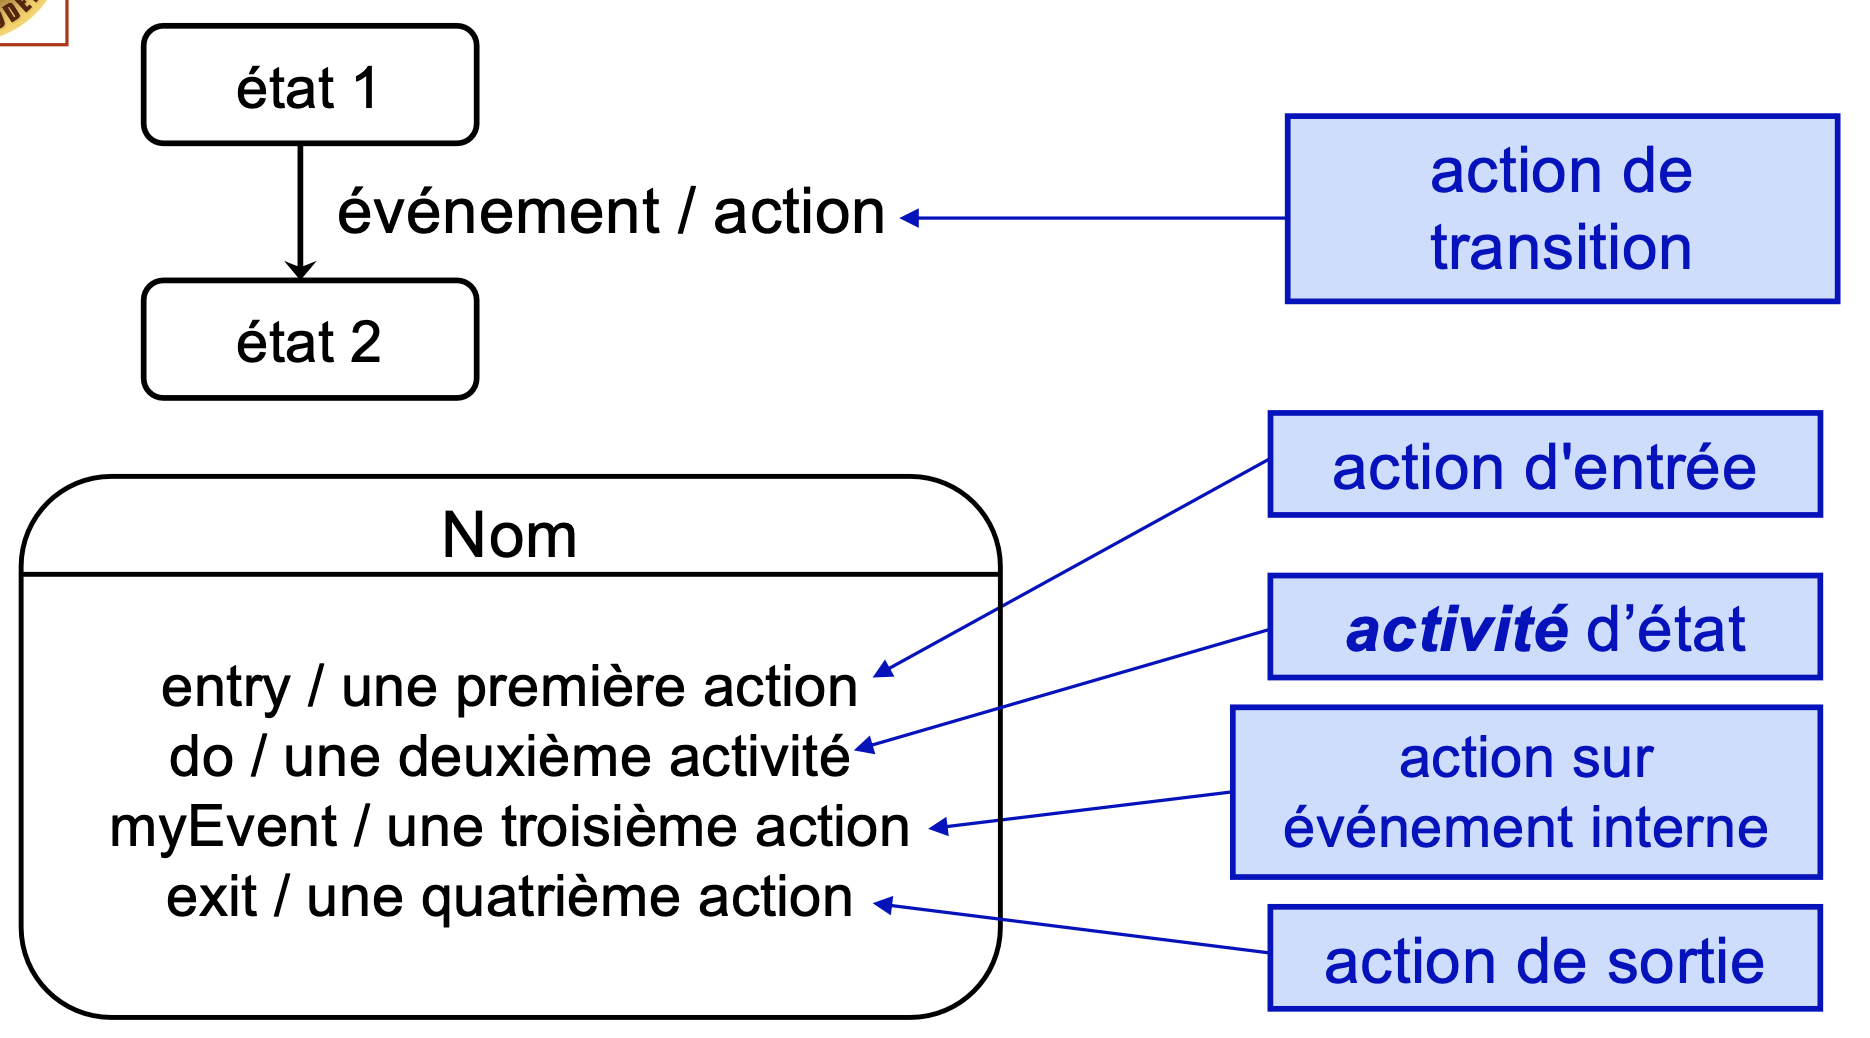
\includegraphics[width=\linewidth]{./Images/Diagrammes/diagram_statechart_actions.png}
  \caption{Les actions associées à entry et exit ne sont pas interruptibles. Les activités associées à do sont interruptibles.}
  \label{fig:actions}
\end{figure}


\begin{table}[H]
\caption{UML fait la distinction entre une activité et une action}
\label{tbl:actionactivite}
\begin{adjustbox}{max width=\textwidth}
\begin{tabular}{l|l|l}
\toprule
\multirow{3}{*}{\textbf{Différences principales}} & Une activité est composée d'actions ordonnées &\\
\cmidrule(lr){2-3}
& \multirow{2}{*}{Une action est une unité d'exécution automatique et non interruptible} & Elle doit se terminer avant qu'une autre action puisse être considérée\\
\cmidrule(lr){3-3}
& & Elle ne peut pas être interrompue par une transition. \\
\cmidrule(lr){1-3}
\textbf{Une action associée à entry ou exit n'a pas de durée} & Elle n'est pas interruptible &\\
\cmidrule(lr){1-3}
\multirow{2}{*}{\textbf{Une activité associée à do prend un temps non négligeable}} & Elle est exécutée pendant que l’objet est dans l’état
donné &\\
\cmidrule(lr){2-3}
& Elle peut être interrompue à tout moment, dès qu’une
transition de sortie d’état est déclenchée &\\
\bottomrule
\end{tabular}
\end{adjustbox}
\end{table}
